% 图 74.6 —— 由 `checks/emit_hand.py` 自动拼出（probe 精测 + prims2 图元分解）
%%
% ⚠ 这是**稿子不是成品**：跑 `checks/checkhand.py 74.6` 看指标 + 看叠合图。
%%
%% ⚠ 待核：
%   · 本图 probe 报出阴影族 2 个 —— **本脚本不生成阴影**（要照原书手写）；prims2 的 strokes 里可能含阴影线，核对时留意别画重
%   · 可疑字形 1 项（空心圈 ⊙ 常被认成字母 o）—— 见文件末
%%
\documentclass[12pt]{standalone}
\usepackage{fontspec}
\setsansfont{Arial}
\newfontfamily\mfallback{DejaVu Sans}
\usepackage{tikz}
\begin{document}
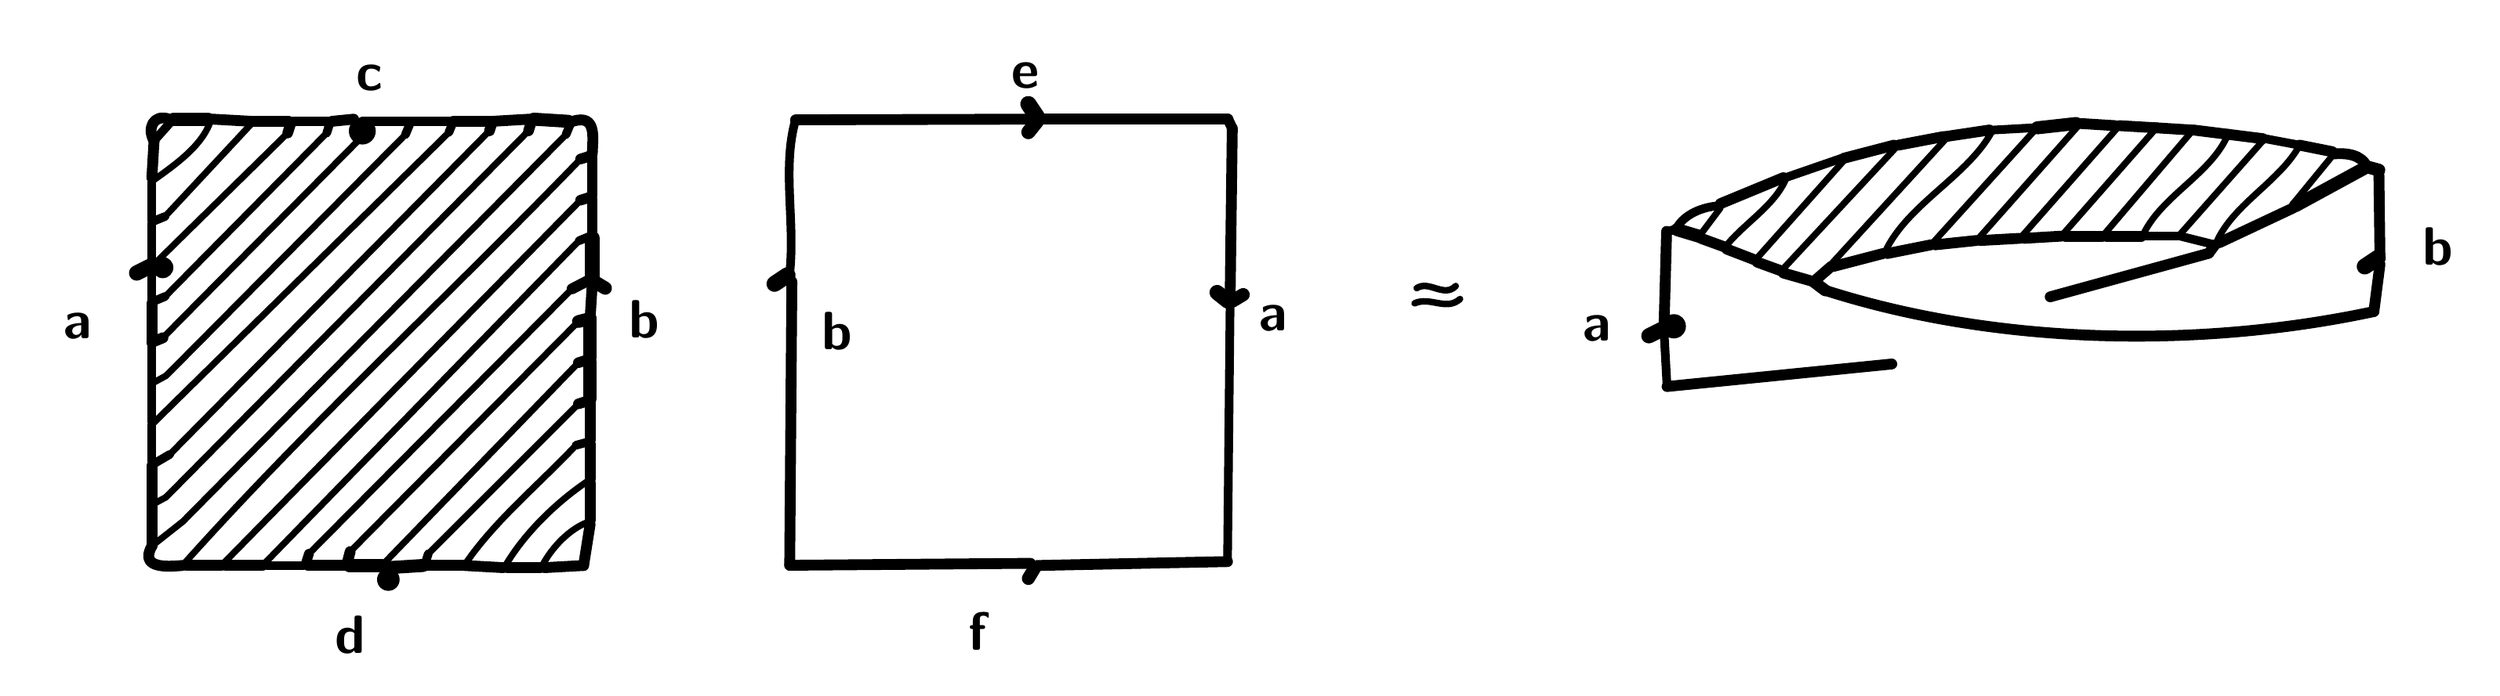
\begin{tikzpicture}[x=1pt, y=-1pt, line width=4.0pt, line cap=round, line join=round]

  %% ════ 填充区（prims2 的 fills）════

  %% ════ 直线段（prims2 的 strokes）════
  \draw[line width=4.0pt] (261.0,194.0) -- (255.5,195.5);
  \draw[line width=4.0pt] (909.0,50.0) -- (927.0,49.0);
  \draw[line width=3.0pt] (948.0,48.0) -- (902.0,100.0);
  \draw[line width=4.9pt] (261.0,156.0) -- (256.6,157.4);
  \draw[line width=3.0pt] (256.6,157.4) -- (167.0,250.0);
  \draw[line width=6.5pt] (464.0,51.0) -- (468.0,46.0);
  \draw[line width=3.0pt] (834.0,112.0) -- (887.0,54.0);
  \draw[line width=5.0pt] (263.0,121.0) -- (262.0,137.0);
  \draw[line width=4.0pt] (61.0,55.0) -- (69.0,46.0);
  \draw[line width=5.0pt] (61.0,55.0) -- (60.0,72.0);
  \draw[line width=4.9pt] (261.0,175.0) -- (256.6,176.4);
  \draw[line width=3.0pt] (256.6,176.4) -- (187.4,245.6);
  \draw[line width=4.0pt] (187.4,245.6) -- (186.0,250.0);
  \draw[line width=5.0pt] (107.0,46.0) -- (123.0,46.0);
  \draw[line width=4.0pt] (125.0,46.0) -- (141.0,46.0);
  \draw[line width=5.0pt] (94.0,251.0) -- (111.0,251.0);
  \draw[line width=7.0pt] (750.0,145.0) -- (756.0,142.0);
  \draw[line width=6.0pt] (467.0,252.0) -- (464.0,257.0);
  \draw[line width=4.0pt] (130.0,251.0) -- (113.0,251.0);
  \draw[line width=5.0pt] (1065.0,60.0) -- (1050.0,57.0);
  \draw[line width=4.0pt] (60.0,92.0) -- (60.0,74.0);
  \draw[line width=6.0pt] (773.0,99.0) -- (763.0,96.0);
  \draw[line width=5.0pt] (1087.0,108.0) -- (1086.5,68.5);
  \draw[line width=5.9pt] (1086.5,68.5) -- (1081.0,67.0);
  \draw[line width=5.0pt] (757.0,141.0) -- (758.2,96.8);
  \draw[line width=4.1pt] (758.2,96.8) -- (762.0,96.0);
  \draw[line width=5.0pt] (965.0,48.0) -- (949.0,47.0);
  \draw[line width=7.1pt] (53.0,116.0) -- (59.0,113.0);
  \draw[line width=5.0pt] (224.0,252.0) -- (239.0,252.0);
  \draw[line width=4.0pt] (60.0,93.0) -- (60.0,111.0);
  \draw[line width=5.0pt] (812.0,116.0) -- (826.0,120.0);
  \draw[line width=5.0pt] (557.0,128.0) -- (558.0,49.2);
  \draw[line width=4.8pt] (558.0,49.2) -- (556.0,45.0);
  \draw[line width=5.0pt] (556.0,45.0) -- (469.0,45.0);
  \draw[line width=3.0pt] (800.0,109.0) -- (840.0,64.0);
  \draw[line width=5.0pt] (106.0,46.0) -- (88.0,45.0);
  \draw[line width=5.0pt] (886.0,53.0) -- (865.0,57.0);
  \draw[line width=3.0pt] (881.0,102.0) -- (928.0,50.0);
  \draw[line width=5.0pt] (882.0,103.0) -- (901.0,101.0);
  \draw[line width=6.0pt] (169.0,252.0) -- (185.0,251.0);
  \draw[line width=5.0pt] (1001.0,50.0) -- (1017.0,52.0);
  \draw[line width=5.0pt] (262.0,211.0) -- (262.0,195.0);
  \draw[line width=5.0pt] (149.0,251.0) -- (132.0,251.0);
  \draw[line width=6.0pt] (86.0,45.0) -- (70.0,45.0);
  \draw[line width=4.0pt] (557.0,130.0) -- (555.8,249.2);
  \draw[line width=5.0pt] (555.8,249.2) -- (468.0,251.0);
  \draw[line width=3.0pt] (156.0,51.0) -- (156.0,54.0);
  \draw[line width=3.0pt] (156.0,54.0) -- (65.1,145.9);
  \draw[line width=5.0pt] (65.1,145.9) -- (60.0,148.0);
  \draw[line width=5.0pt] (262.0,230.0) -- (262.0,213.0);
  \draw[line width=5.0pt] (234.0,45.0) -- (217.0,46.0);
  \draw[line width=4.0pt] (199.0,46.0) -- (180.0,46.0);
  \draw[line width=5.0pt] (199.0,46.0) -- (217.0,46.0);
  \draw[line width=4.0pt] (199.0,46.0) -- (196.9,51.1);
  \draw[line width=3.0pt] (196.9,51.1) -- (61.0,185.0);
  \draw[line width=4.9pt] (217.0,46.0) -- (215.6,50.4);
  \draw[line width=3.0pt] (215.6,50.4) -- (68.3,199.7);
  \draw[line width=4.0pt] (68.3,199.7) -- (61.0,204.0);
  \draw[line width=6.1pt] (264.0,120.0) -- (269.0,123.0);
  \draw[line width=5.0pt] (186.0,251.0) -- (204.0,251.0);
  \draw[line width=6.1pt] (563.0,126.0) -- (558.0,129.0);
  \draw[line width=5.0pt] (204.0,251.0) -- (222.0,252.0);
  \draw[line width=7.4pt] (353.0,117.0) -- (347.0,121.0);
  \draw[line width=3.0pt] (783.0,86.0) -- (774.0,98.0);
  \draw[line width=3.0pt] (995.0,98.0) -- (1033.0,55.0);
  \draw[line width=5.0pt] (467.0,45.0) -- (356.7,45.3);
  \draw[line width=7.4pt] (464.0,38.0) -- (468.0,44.0);
  \draw[line width=5.0pt] (959.0,99.0) -- (942.0,99.0);
  \draw[line width=5.0pt] (977.0,99.0) -- (961.0,99.0);
  \draw[line width=5.0pt] (60.0,205.0) -- (60.0,223.0);
  \draw[line width=4.0pt] (61.0,129.0) -- (66.2,126.8);
  \draw[line width=3.0pt] (66.2,126.8) -- (140.6,51.4);
  \draw[line width=4.0pt] (140.6,51.4) -- (142.0,47.0);
  \draw[line width=7.0pt] (263.0,100.0) -- (263.0,118.0);
  \draw[line width=4.0pt] (157.0,46.0) -- (179.0,46.0);
  \draw[line width=4.0pt] (60.0,186.0) -- (60.0,203.0);
  \draw[line width=6.0pt] (262.0,157.0) -- (262.0,174.0);
  \draw[line width=3.0pt] (922.0,99.0) -- (966.0,49.0);
  \draw[line width=5.0pt] (940.0,99.0) -- (923.0,100.0);
  \draw[line width=5.0pt] (60.0,148.0) -- (60.0,130.0);
  \draw[line width=4.0pt] (60.0,148.0) -- (60.0,167.0);
  \draw[line width=3.0pt] (812.0,114.0) -- (864.0,58.0);
  \draw[line width=5.0pt] (262.0,119.0) -- (253.7,123.3);
  \draw[line width=3.0pt] (253.7,123.3) -- (132.4,245.6);
  \draw[line width=4.5pt] (132.4,245.6) -- (131.0,250.0);
  \draw[line width=5.0pt] (262.0,176.0) -- (262.0,193.0);
  \draw[line width=4.9pt] (262.0,81.0) -- (257.6,82.4);
  \draw[line width=3.0pt] (257.6,82.4) -- (93.0,250.0);
  \draw[line width=5.0pt] (143.0,46.0) -- (153.0,45.0);
  \draw[line width=5.0pt] (834.0,113.0) -- (826.0,120.0);
  \draw[line width=3.0pt] (60.0,167.0) -- (66.6,163.4);
  \draw[line width=3.0pt] (66.6,163.4) -- (176.9,52.1);
  \draw[line width=4.0pt] (176.9,52.1) -- (179.0,47.0);
  \draw[line width=4.0pt] (60.0,167.0) -- (60.0,185.0);
  \draw[line width=5.0pt] (785.0,104.0) -- (774.0,100.0);
  \draw[line width=6.0pt] (166.0,251.0) -- (151.0,251.0);
  \draw[line width=4.0pt] (60.0,129.0) -- (60.0,114.0);
  \draw[line width=3.0pt] (106.0,47.0) -- (66.1,89.9);
  \draw[line width=4.0pt] (66.1,89.9) -- (61.0,92.0);
  \draw[line width=4.9pt] (262.0,62.0) -- (257.6,63.4);
  \draw[line width=4.0pt] (1050.0,57.0) -- (1034.0,54.0);
  \draw[line width=6.0pt] (929.0,49.0) -- (947.0,47.0);
  \draw[line width=7.0pt] (551.0,125.0) -- (556.0,129.0);
  \draw[line width=7.4pt] (1080.0,113.0) -- (1086.0,109.0);
  \draw[line width=5.0pt] (907.0,50.0) -- (887.0,53.0);
  \draw[line width=6.0pt] (1081.0,67.0) -- (1048.0,85.0);
  \draw[line width=5.0pt] (150.0,250.0) -- (151.4,244.6);
  \draw[line width=3.0pt] (151.4,244.6) -- (256.6,138.4);
  \draw[line width=5.9pt] (256.6,138.4) -- (262.0,137.0);
  \draw[line width=5.0pt] (241.0,252.0) -- (259.0,251.0);
  \draw[line width=5.0pt] (259.0,251.0) -- (262.0,232.0);
  \draw[line width=4.0pt] (813.0,72.0) -- (839.0,63.0);
  \draw[line width=3.0pt] (960.0,98.0) -- (1000.0,51.0);
  \draw[line width=5.5pt] (826.0,120.0) -- (831.3,124.0);
  \draw[line width=5.0pt] (1084.2,133.8) -- (1087.0,112.0);
  \draw[line width=5.0pt] (92.0,251.0) -- (76.0,251.0);
  \draw[line width=5.0pt] (799.0,110.0) -- (786.0,105.0);
  \draw[line width=4.9pt] (235.0,46.0) -- (233.6,50.4);
  \draw[line width=3.0pt] (233.6,50.4) -- (66.5,219.5);
  \draw[line width=3.0pt] (66.5,219.5) -- (60.0,223.0);
  \draw[line width=5.0pt] (840.0,63.0) -- (863.0,57.0);
  \draw[line width=5.0pt] (783.0,84.0) -- (812.0,72.0);
  \draw[line width=5.0pt] (263.0,98.0) -- (263.0,82.0);
  \draw[line width=3.0pt] (62.0,111.0) -- (122.6,51.4);
  \draw[line width=4.9pt] (122.6,51.4) -- (124.0,47.0);
  \draw[line width=5.0pt] (860.0,107.0) -- (880.0,103.0);
  \draw[line width=5.0pt] (1000.0,50.0) -- (984.0,49.0);
  \draw[line width=4.0pt] (1011.0,103.0) -- (995.0,99.0);
  \draw[line width=4.9pt] (1011.0,103.0) -- (1008.1,106.9);
  \draw[line width=5.0pt] (1008.1,106.9) -- (935.0,127.0);
  \draw[line width=3.0pt] (941.0,98.0) -- (984.0,49.0);
  \draw[line width=5.0pt] (1047.0,86.0) -- (1013.0,102.0);
  \draw[line width=6.0pt] (262.0,155.0) -- (262.0,137.0);
  \draw[line width=3.0pt] (112.0,250.0) -- (256.9,101.1);
  \draw[line width=4.0pt] (256.9,101.1) -- (262.0,99.0);
  \draw[line width=5.0pt] (1017.0,52.0) -- (1033.0,54.0);
  \draw[line width=4.0pt] (994.0,99.0) -- (979.0,99.0);
  \draw[line width=5.0pt] (984.0,49.0) -- (967.0,48.0);
  \draw[line width=5.0pt] (263.0,63.0) -- (263.0,80.0);
  \draw[line width=5.0pt] (858.0,107.0) -- (835.0,113.0);
  \draw[line width=6.0pt] (236.0,45.0) -- (252.0,46.0);
  \draw[line width=4.0pt] (757.0,143.0) -- (758.4,168.4);
  \draw[line width=5.0pt] (758.4,168.4) -- (862.0,158.0);
  \draw[line width=5.0pt] (811.0,115.0) -- (800.0,111.0);
  \draw[line width=5.0pt] (903.0,101.0) -- (921.0,100.0);
  \draw[line width=5.0pt] (465.0,250.0) -- (354.0,250.9);
  \draw[line width=5.0pt] (354.0,250.9) -- (355.0,120.0);
  \draw[line width=4.0pt] (253.0,47.0) -- (250.9,52.1);
  \draw[line width=3.0pt] (250.9,52.1) -- (74.3,230.7);
  \draw[line width=3.0pt] (74.3,230.7) -- (60.0,242.0);
  \draw[line width=3.0pt] (1065.0,62.0) -- (1047.0,84.0);
  \draw[line width=5.0pt] (60.0,223.0) -- (60.0,242.0);

  %% ════ 曲线（prims2 的 curves —— 三段式，坐标同为 (y,x)）════
  \draw[line width=3.0pt] (255.5,195.5) .. controls (238.3,213.8) and (217.5,230.8) .. (204.0,251.0);
  \draw[line width=4.0pt] (763.0,95.0) .. controls (766.6,88.7) and (775.0,85.5) .. (782.0,85.0);
  \draw[line width=5.0pt] (61.0,55.0) .. controls (57.7,49.4) and (60.6,42.4) .. (68.0,45.0);
  \draw[line width=3.0pt] (223.0,251.0) .. controls (231.8,236.1) and (246.4,221.8) .. (261.0,212.0);
  \draw[line width=3.0pt] (813.0,73.0) .. controls (807.8,84.8) and (794.5,92.8) .. (786.0,103.0);
  \draw[line width=3.0pt] (87.0,46.0) .. controls (83.1,57.4) and (70.6,66.1) .. (61.0,73.0);
  \draw[line width=5.0pt] (74.0,251.0) .. controls (66.9,251.6) and (54.2,252.5) .. (60.0,242.0);
  \draw[line width=3.0pt] (859.0,106.0) .. controls (869.6,84.0) and (896.4,71.7) .. (908.0,51.0);
  \draw[line width=4.0pt] (356.7,45.3) .. controls (350.4,67.2) and (356.6,92.5) .. (354.0,116.0);
  \draw[line width=5.0pt] (1066.0,61.0) .. controls (1071.7,60.6) and (1078.4,61.3) .. (1081.0,67.0);
  \draw[line width=3.0pt] (1012.0,101.0) .. controls (1020.1,83.8) and (1041.0,73.5) .. (1050.0,57.0);
  \draw[line width=3.0pt] (257.6,63.4) .. controls (197.6,125.7) and (132.7,185.5) .. (75.0,250.0);
  \draw[line width=5.0pt] (254.0,46.0) .. controls (265.2,42.5) and (263.2,53.5) .. (263.0,61.0);
  \draw[line width=3.0pt] (661.0,122.0) .. controls (655.6,127.6) and (648.7,119.2) .. (643.0,123.0);
  \draw[line width=5.0pt] (831.3,124.0) .. controls (909.5,149.1) and (1002.7,151.2) .. (1084.2,133.8);
  \draw[line width=3.0pt] (240.0,251.0) .. controls (244.2,242.9) and (252.4,234.1) .. (261.0,231.0);
  \draw[line width=3.0pt] (663.0,128.0) .. controls (656.7,133.7) and (649.2,126.7) .. (642.0,130.0);
  \draw[line width=3.0pt] (1017.0,52.0) .. controls (1009.2,70.3) and (986.7,80.1) .. (978.0,98.0);

  %% ════ 实心点 ════
  \fill (157.0,50.5) circle (6.2);
  \fill (65.0,113.5) circle (4.9);
  \fill (761.5,140.6) circle (5.6);
  \fill (169.0,257.5) circle (5.2);

  %% ════ 标签（probe 直接给的 \node 行）════
  %% ⚠ 全部补了 fill=white：文字在最上层，否则与曲线交叉干扰
     \node[anchor=center,inner sep=0pt,fill=white,font=\fontsize{31.4}{39.3}\selectfont] at (462.8,25.1) {\textsf{\textbf{\textit{e}}}};   % box(453,15,16,17)
     \node[anchor=center,inner sep=0pt,fill=white,font=\fontsize{30.5}{38.1}\selectfont] at (160.3,26.0) {\textsf{\textbf{\textit{c}}}};   % box(152,16,15,17)
     \node[anchor=center,inner sep=0pt,fill=white,font=\fontsize{30.7}{38.3}\selectfont] at (1113.8,103.8) {\textsf{\textbf{\textit{b}}}};   % box(1104,91,17,23)
     \node[anchor=center,inner sep=0pt,fill=white,font=\fontsize{30.0}{37.5}\selectfont] at (286.8,137.2) {\textsf{\textbf{\textit{b}}}};   % box(277,125,17,22)
     \node[anchor=center,inner sep=0pt,fill=white,font=\fontsize{32.0}{40.0}\selectfont] at (577.1,137.1) {\textsf{\textbf{\textit{a}}}};   % box(568,127,16,17)
     \node[anchor=center,inner sep=0pt,fill=white,font=\fontsize{32.9}{41.1}\selectfont] at (26.1,140.6) {\textsf{\textbf{\textit{a}}}};   % box(17,130,16,18)
     \node[anchor=center,inner sep=0pt,fill=white,font=\fontsize{30.7}{38.3}\selectfont] at (375.8,142.8) {\textsf{\textbf{\textit{b}}}};   % box(366,130,17,23)
     \node[anchor=center,inner sep=0pt,fill=white,font=\fontsize{32.9}{41.1}\selectfont] at (726.1,141.6) {\textsf{\textbf{\textit{a}}}};   % box(717,131,16,18)
     \node[anchor=center,inner sep=0pt,fill=white,font=\fontsize{30.7}{38.3}\selectfont] at (151.3,282.8) {\textsf{\textbf{\textit{d}}}};   % box(141,270,18,23)
     \node[anchor=center,inner sep=0pt,fill=white,font=\fontsize{29.7}{37.2}\selectfont] at (441.5,281.5) {\textsf{\textbf{\textit{f}}}};   % box(435,270,12,22)

  % 钉死画布：否则超出的图元/控制点会把页面撑大，1:1 回比就失准
  \pgfresetboundingbox
  \path[use as bounding box] (0,0) rectangle (1132,301);
\end{tikzpicture}
\end{document}

% ⚠ 待核清单（probe 拿不准，人眼过一遍）：
%   · 未识别/跳过：⑤ 跳过/未识别的字形
